

%\section{État de l'art}
\section{Méthodes de projection de liquides}\label{sec:etat de lart}
\subsection{Bombe spray}
Pour constituer des écrans de turbulence aisément, l'approche de la bombe de spray pour les cheveux, ou de laque transparente pour surfaces a été employée.
\begin{figure}[H]
    \centering
    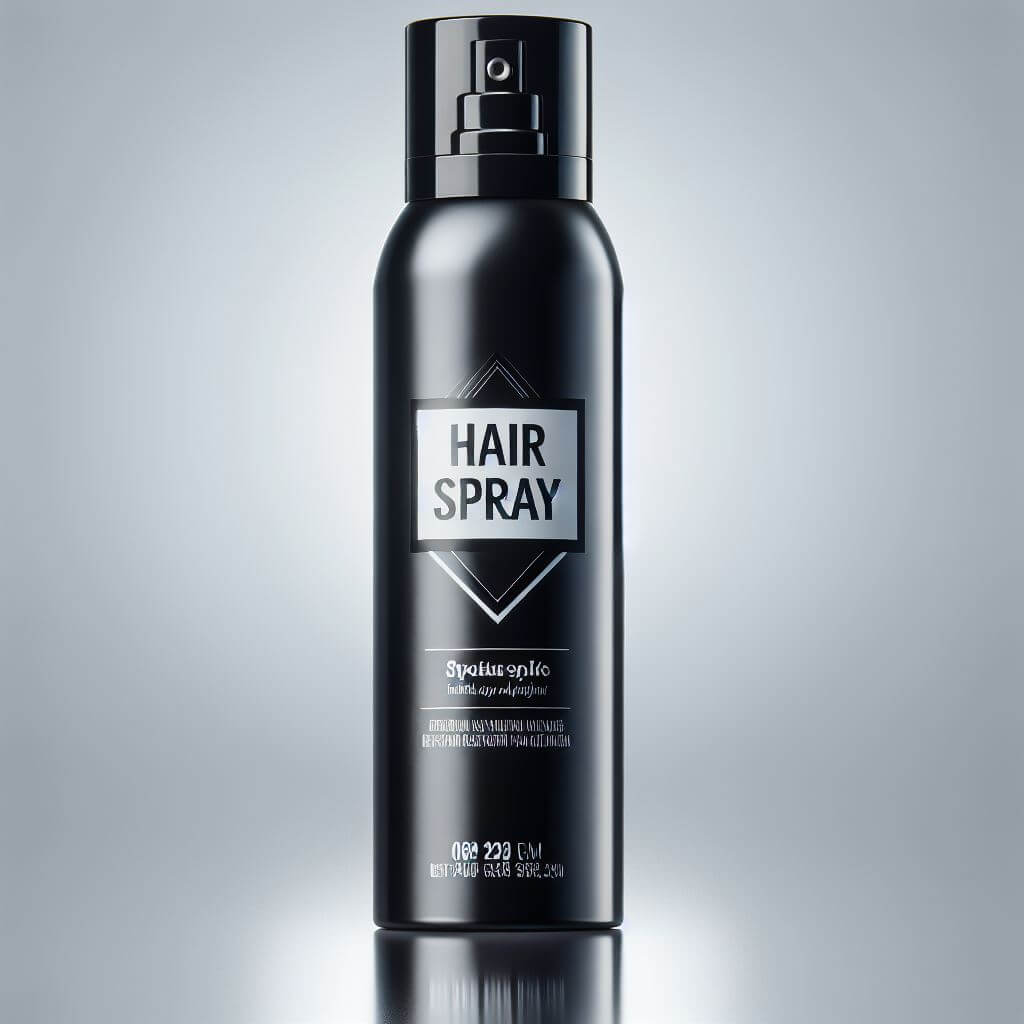
\includegraphics[width=0.3\textwidth,trim={4cm 0 4cm 0},clip]{assets/figures/etat_art/airspray.jpeg}

    \caption{Bombe de laque (IA)}
\end{figure}
Cette solution étant assez sommaire et peu reproductible, elle a été abandonnée au profit de méthodes plus contrôlables.
La durée du "pschit" est sujette à l'erreur humaine, la quantité de liquide projetée
dépend directement de la durée d'appui, mais aussi de la pression du gaz de la bombe, cette
dernière diminuant au fil des usages et variant en fonction de la température et de l'altitude,
explique pourquoi cette solution ne fut pas sélectionnée.

% Please add the following required packages to your document preamble:
% \usepackage[table,xcdraw]{xcolor}
% Beamer presentation requires \usepackage{colortbl} instead of \usepackage[table,xcdraw]{xcolor}
\begin{table}[H]
    \centering
    \begin{tabular}{|c|c|lll}
        \cline{1-2}
        Avantages                                 & Inconvénients                                                          &  &  & \\ \cline{1-2}
        \cellcolor[HTML]{67FD9A}Abordable         & \cellcolor[HTML]{FD6864}Durée de "pschit" hasardeuse                   &  &  & \\ \cline{1-2}
        \cellcolor[HTML]{67FD9A}trouvable partout & \cellcolor[HTML]{FD6864}Dépendante de la température et de la pression &  &  & \\ \cline{1-2}
                                                  & \cellcolor[HTML]{FD6864}Très artisanal                                 &  &  & \\ \cline{1-2}
    \end{tabular}
    \caption{Résumé des avantages et inconvénients du spray}
    \label{tab:hair_spray_table}
\end{table}

\newpage
\subsection{Aérographe} \label{section_aerographe}
L'aérographe est un pistolet à peinture miniature similaire à un pistolet généralement utilisé pour les travaux de précision
à peinture utilisé par les carrossiers.
Ces derniers sont généralement alimentés à l'aide d'un compresseur et peuvent projeter plusieurs médiums.

\begin{figure}[H]
    \centering
    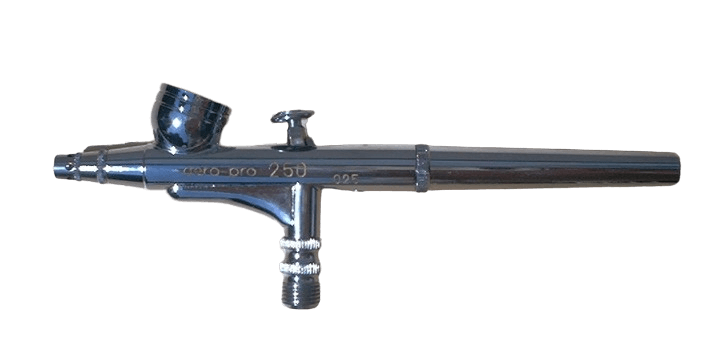
\includegraphics[width=0.8\textwidth]{assets/figures/etat_art/airbrush.png}
    \caption[Aérographe]{Aérographe \cite{airbrush_pics}\footnotemark}
\end{figure}
\footnotetext{\url{http://ingo-karkat.de/textilepainting/About\%20used\%20tools/index.html}}

L'aérographe repose sur l'effet venturi, l'air comprimé entraine le liquide à projeter dans l'embouchure assez fine de l'outil
transformant ce dernier en gouttelettes plus ou moins fines en fonction du réglage de l'aiguille de l'outil.

\begin{figure}[H]
    \centering
    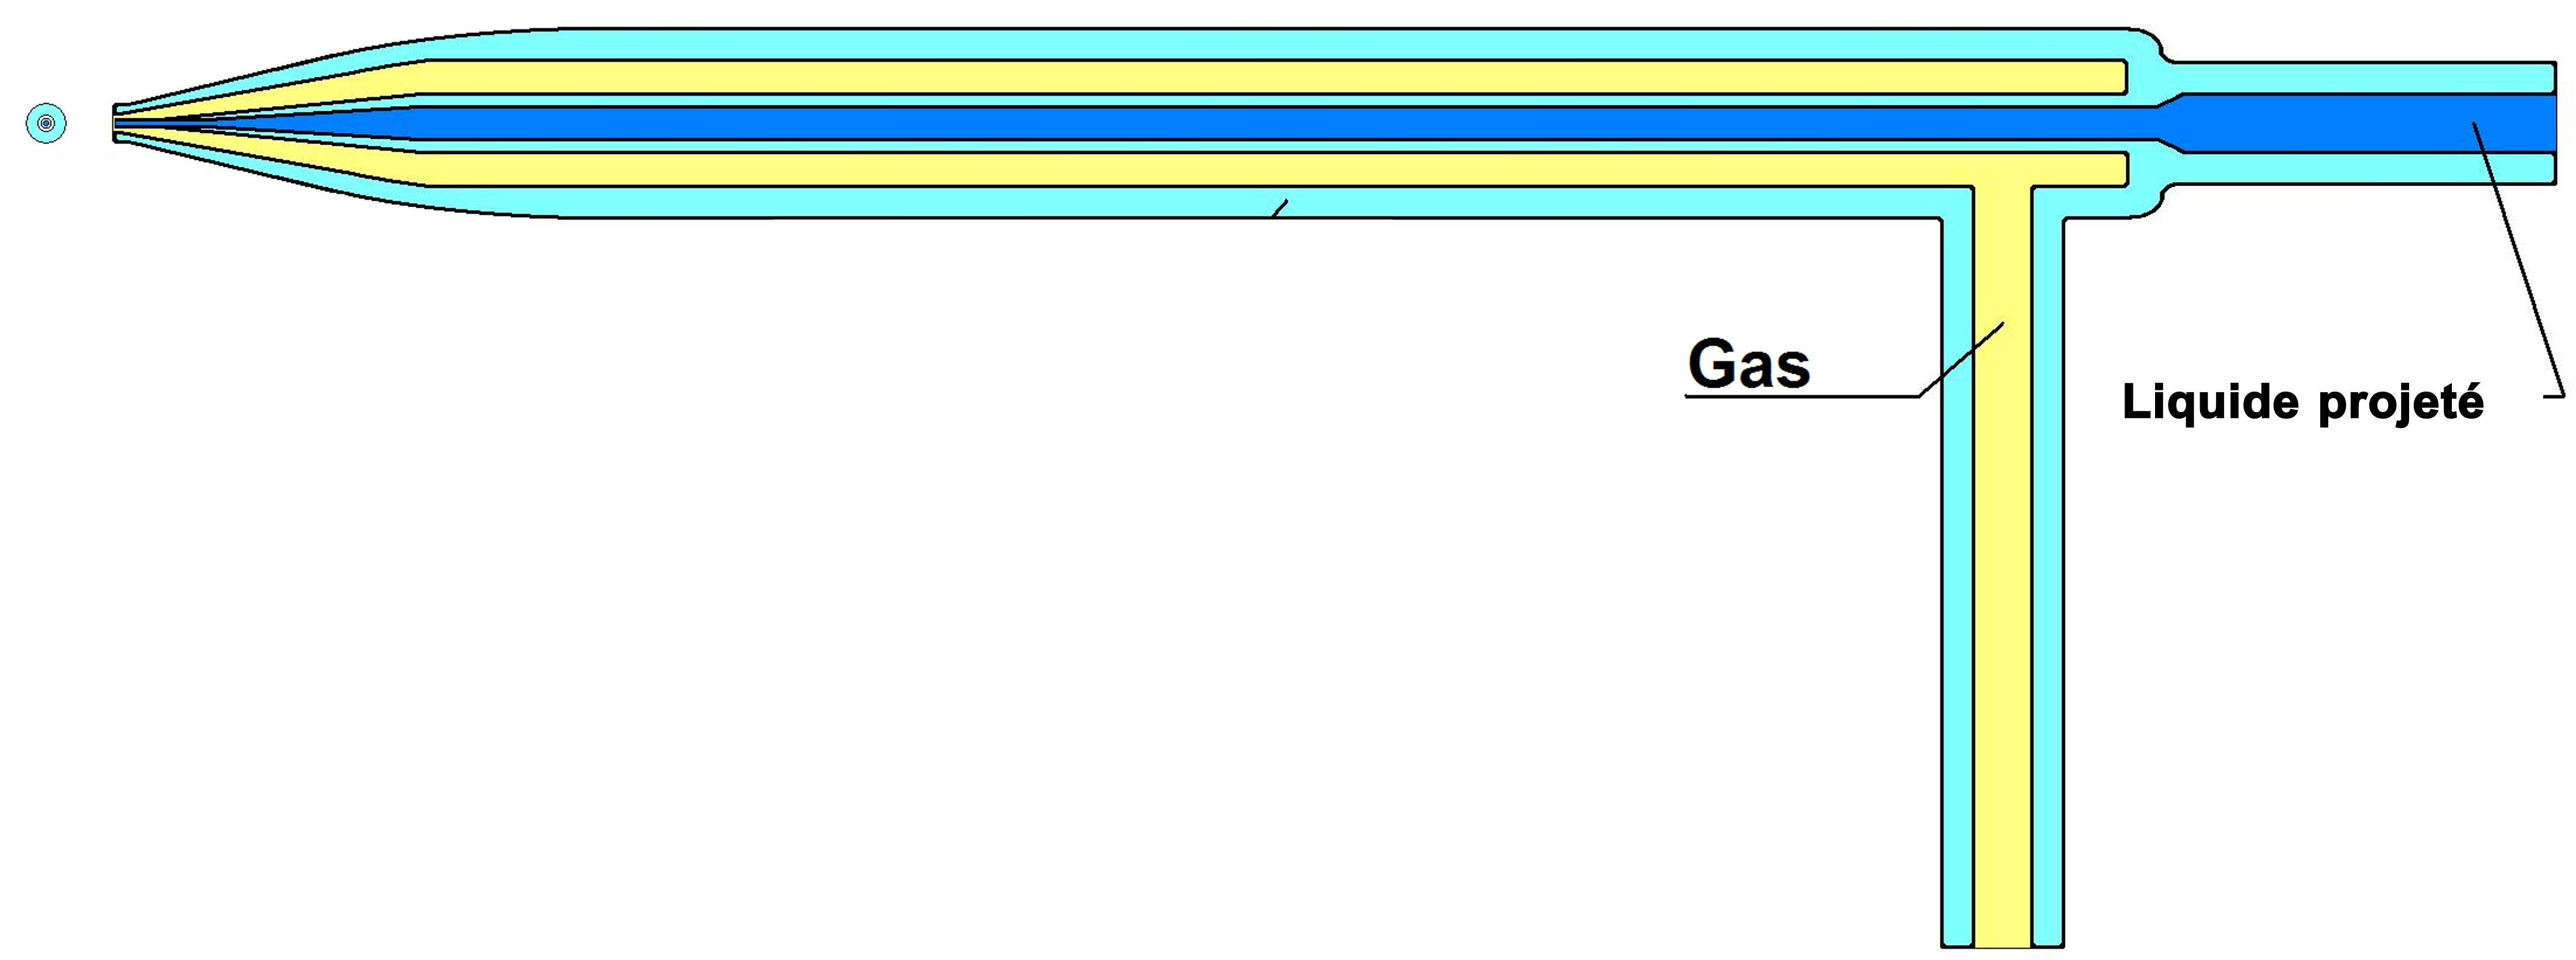
\includegraphics[width=0.6\textwidth]{assets/figures/etat_art/effet_venturi_aerographe.jpg}
    \caption[Effet venturi dans un aérographe]{Effet venturi dans aérographe \cite{venturi_airbrush}\footnotemark}
\end{figure}
\footnotetext{\url{https://upload.wikimedia.org/wikipedia/commons/1/1e/Nebulizzatoe\_concentrico.png}}

C'est la solution de projection sélectionnée dans la machine actuelle, il a pour avantage, d'être réglable assez finement
et de ne nécessiter qu'un compresseur, le critère de sélection principal lors du choix effectué par le concepteur de la machine
était la disponibilité de l'outil de façon rapide en l'empruntant à un tiers.

% Please add the following required packages to your document preamble:
% \usepackage[table,xcdraw]{xcolor}
% Beamer presentation requires \usepackage{colortbl} instead of \usepackage[table,xcdraw]{xcolor}
\begin{table}[H]
    \centering
    \begin{tabular}{|c|c|lll}
        \cline{1-2}
        Avantages                                                                                            & Inconvénients                                     &  &  & \\ \cline{1-2}
        \cellcolor[HTML]{67FD9A}Non influencé par l'environnement                                            & \cellcolor[HTML]{FD6864}Montage actuel capricieux &  &  & \\ \cline{1-2}
        \cellcolor[HTML]{67FD9A}Motorisable -\textgreater reproductible                                      & \cellcolor[HTML]{FFFFFF}                          &  &  & \\ \cline{1-2}
        \cellcolor[HTML]{67FD9A}Beaucoup de possibilités de modifier la brumisation                          & \cellcolor[HTML]{FFFFFF}                          &  &  & \\ \cline{1-2}
        \multicolumn{1}{|l|}{\cellcolor[HTML]{67FD9A}Possibilité de contrôler la composition de l'acrylique} & \multicolumn{1}{l|}{}                             &  &  & \\ \cline{1-2}
        \multicolumn{1}{|l|}{\cellcolor[HTML]{67FD9A}Bouton qui bloque l'air intégré}                        & \multicolumn{1}{l|}{}                             &  &  & \\ \cline{1-2}
    \end{tabular}
    \caption{Résumé des avantages et inconvénients de l'aérographe}
    \label{tab:aerographe_table}
\end{table}
\subsection{Atomiseurs pneumatiques}
Les atomiseurs pneumatiques reposent sur le même principe de fonctionnement que l'aérographe de la \autoref{section_aerographe}, donc avec effet
venturi et une aiguille pour régler la taille des gouttelettes.
\begin{figure}[H]
    \centering
    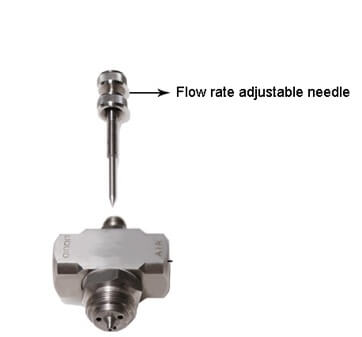
\includegraphics[width=0.5\textwidth]{assets/figures/etat_art/atomizing_nozzle.jpg}
    \caption[Buse d'atomisation pneumatique]{Buse d'atomisation pneumatique \autocite{photo_buse_atomisation}\footnotemark}
\end{figure}
\footnotetext{\url{https://www.nozzlespray.com/uploads/allimg/220310/atomizingfogspraynozzlefordisinfection.jpg}}

Ces buses d'atomisation à air comprimé sont utilisées dans l'industrie pour recouvrir des surfaces (peinture), nettoyer avec de l'eau, dans la confection d'aliments et bien d'autres:
\begin{figure}[H]
    \centering
    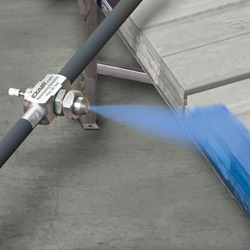
\includegraphics[width=0.5\textwidth]{assets/figures/etat_art/buse spray.jpeg}
    \caption[Exemple d'application d'une buse d'atomisation]{Exemple d'application d'une buse d'atomisation \autocite{exemple_application_buse}\footnotemark}
\end{figure}
\footnotetext{\url{https://english.exair.com/images/atom/IntMix-2\_250sq.png}}
\newpage
Elles permettent un choix de formes de projection assez vaste :
\begin{figure}[H]
    \centering
    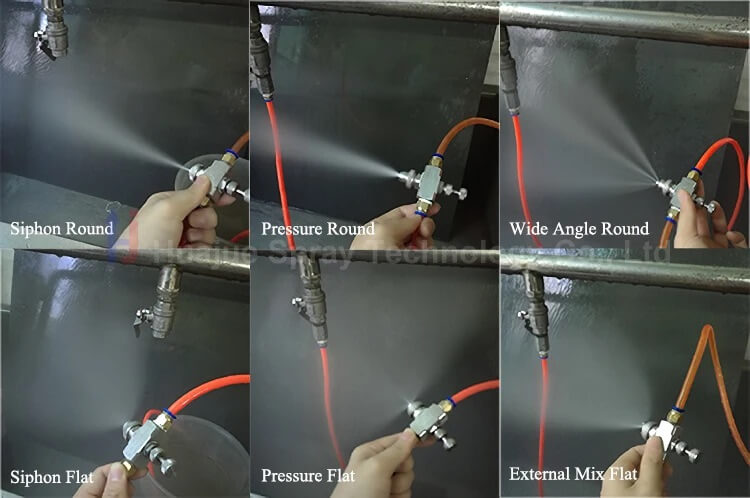
\includegraphics[width=0.9\textwidth]{assets/figures/etat_art/spray_patterns_example.jpeg}
    \caption[Exemples de différents "motifs" de spray]{Exemples de différents "motifs" de spray \autocite{Exemples_spray_patterns}\footnotemark}
\end{figure}
\footnotetext{\url{https://ae01.alicdn.com/kf/H428bb75251884fee8f19beffbbd38cfdp.jpg}}
C'est une piste de solution intéressante, elle fait déjà ses preuves dans plusieurs industries différentes.
L'activation du spray devra se faire de façon externe avec une électrovanne par exemple. Concernant la gestion de la taille
des gouttelettes, il faudra automatiser l'actionnement de l'aiguille. Concernant un point important pour ce type de matériel industriel, le prix,
des fournisseurs chinois pratiqueront des prix dans l'ordre de 10-20 frs, tandis que des fournisseurs traditionnels se situent plus dans les 300-800 frs. Il ne semble
pas y avoir de milieu de gamme.

% Please add the following required packages to your document preamble:
% \usepackage{graphicx}
% \usepackage[table,xcdraw]{xcolor}
% Beamer presentation requires \usepackage{colortbl} instead of \usepackage[table,xcdraw]{xcolor}
\begin{table}[H]
    \centering
    \resizebox{\textwidth}{!}{%
        \begin{tabular}{|c|c|lll}
            \cline{1-2}
            Avantages                                                                                            & Inconvénients                                                  &  &  & \\ \cline{1-2}
            \cellcolor[HTML]{67FD9A}Non influencé par l'environnement                                            & \cellcolor[HTML]{FD6864}Pas de bouton de blocage du flux d'air &  &  & \\ \cline{1-2}
            \cellcolor[HTML]{67FD9A}Motorisable -\textgreater reproductible                                      & \cellcolor[HTML]{FD6864}Classes de prix non régulières         &  &  & \\ \cline{1-2}
            \cellcolor[HTML]{67FD9A}Beaucoup de possibilités de modifier la brumisation                          & \cellcolor[HTML]{FFFFFF}                                       &  &  & \\ \cline{1-2}
            \multicolumn{1}{|l|}{\cellcolor[HTML]{67FD9A}Possibilité de contrôler la composition de l'acrylique} & \multicolumn{1}{l|}{}                                          &  &  & \\ \cline{1-2}
            \multicolumn{1}{|l|}{\cellcolor[HTML]{67FD9A}Solution utilisée dans l'industrie}                     & \multicolumn{1}{l|}{}                                          &  &  & \\ \cline{1-2}
            \multicolumn{1}{|l|}{\cellcolor[HTML]{67FD9A}Méthode de montage standardisée}                        & \multicolumn{1}{l|}{}                                          &  &  & \\ \cline{1-2}
        \end{tabular}%
    }
    \caption{Résumé des avantages et inconvénients de l'atomiseur pneumatique}
    \label{tab:atomiseur_pneumatique_table}
\end{table}

\newpage

\section{Liquides à projeter}
Dans cette partie de l'état de l'art, nous allons passer en revue les matériaux projetables sur les disques en acrylique.
La boîte de matériel du concepteur de la machine d'origine contenait déjà certains matériaux de cette section.

Avant de commencer à présenter différentes pistes, il est important de noter, que l'ensemble des liquides proposés auront une finition brillante
quand ils seront totalement secs, en effet, une finition matte absorberait la lumière ou du moins la diffuserait dans son épaisseur, tandis qu'un aspect brillant
ne réfléchira qu'une faible partie de la lumière travsersant la surface, tout en restant transparente et donc perméable à la lumière !
\subsection{Laque transparente d'acrylique à l'eau de Lascaux}

C'est un des matériaux de projection fournis avec le matériel au début du projet, il est produit par la marque \href{https://lascaux.ch/en/start}{Lascaux}\footnotemark \footnotetext{\url{https://lascaux.ch/en/start}}.
C'est une laque transparente résistante aux UV utilisée pour protéger des peintures à base d'acrylique. Elle est décrite sur la \href{https://lascaux.ch/lascaux-varnishes-and-fixative/lascaux-transparent-varnish-1-uv-gloss}{page produit}\footnotemark
comme \say{Hautement transparente et claire comme du cristal}:

\begin{figure}[H]
    \centering
    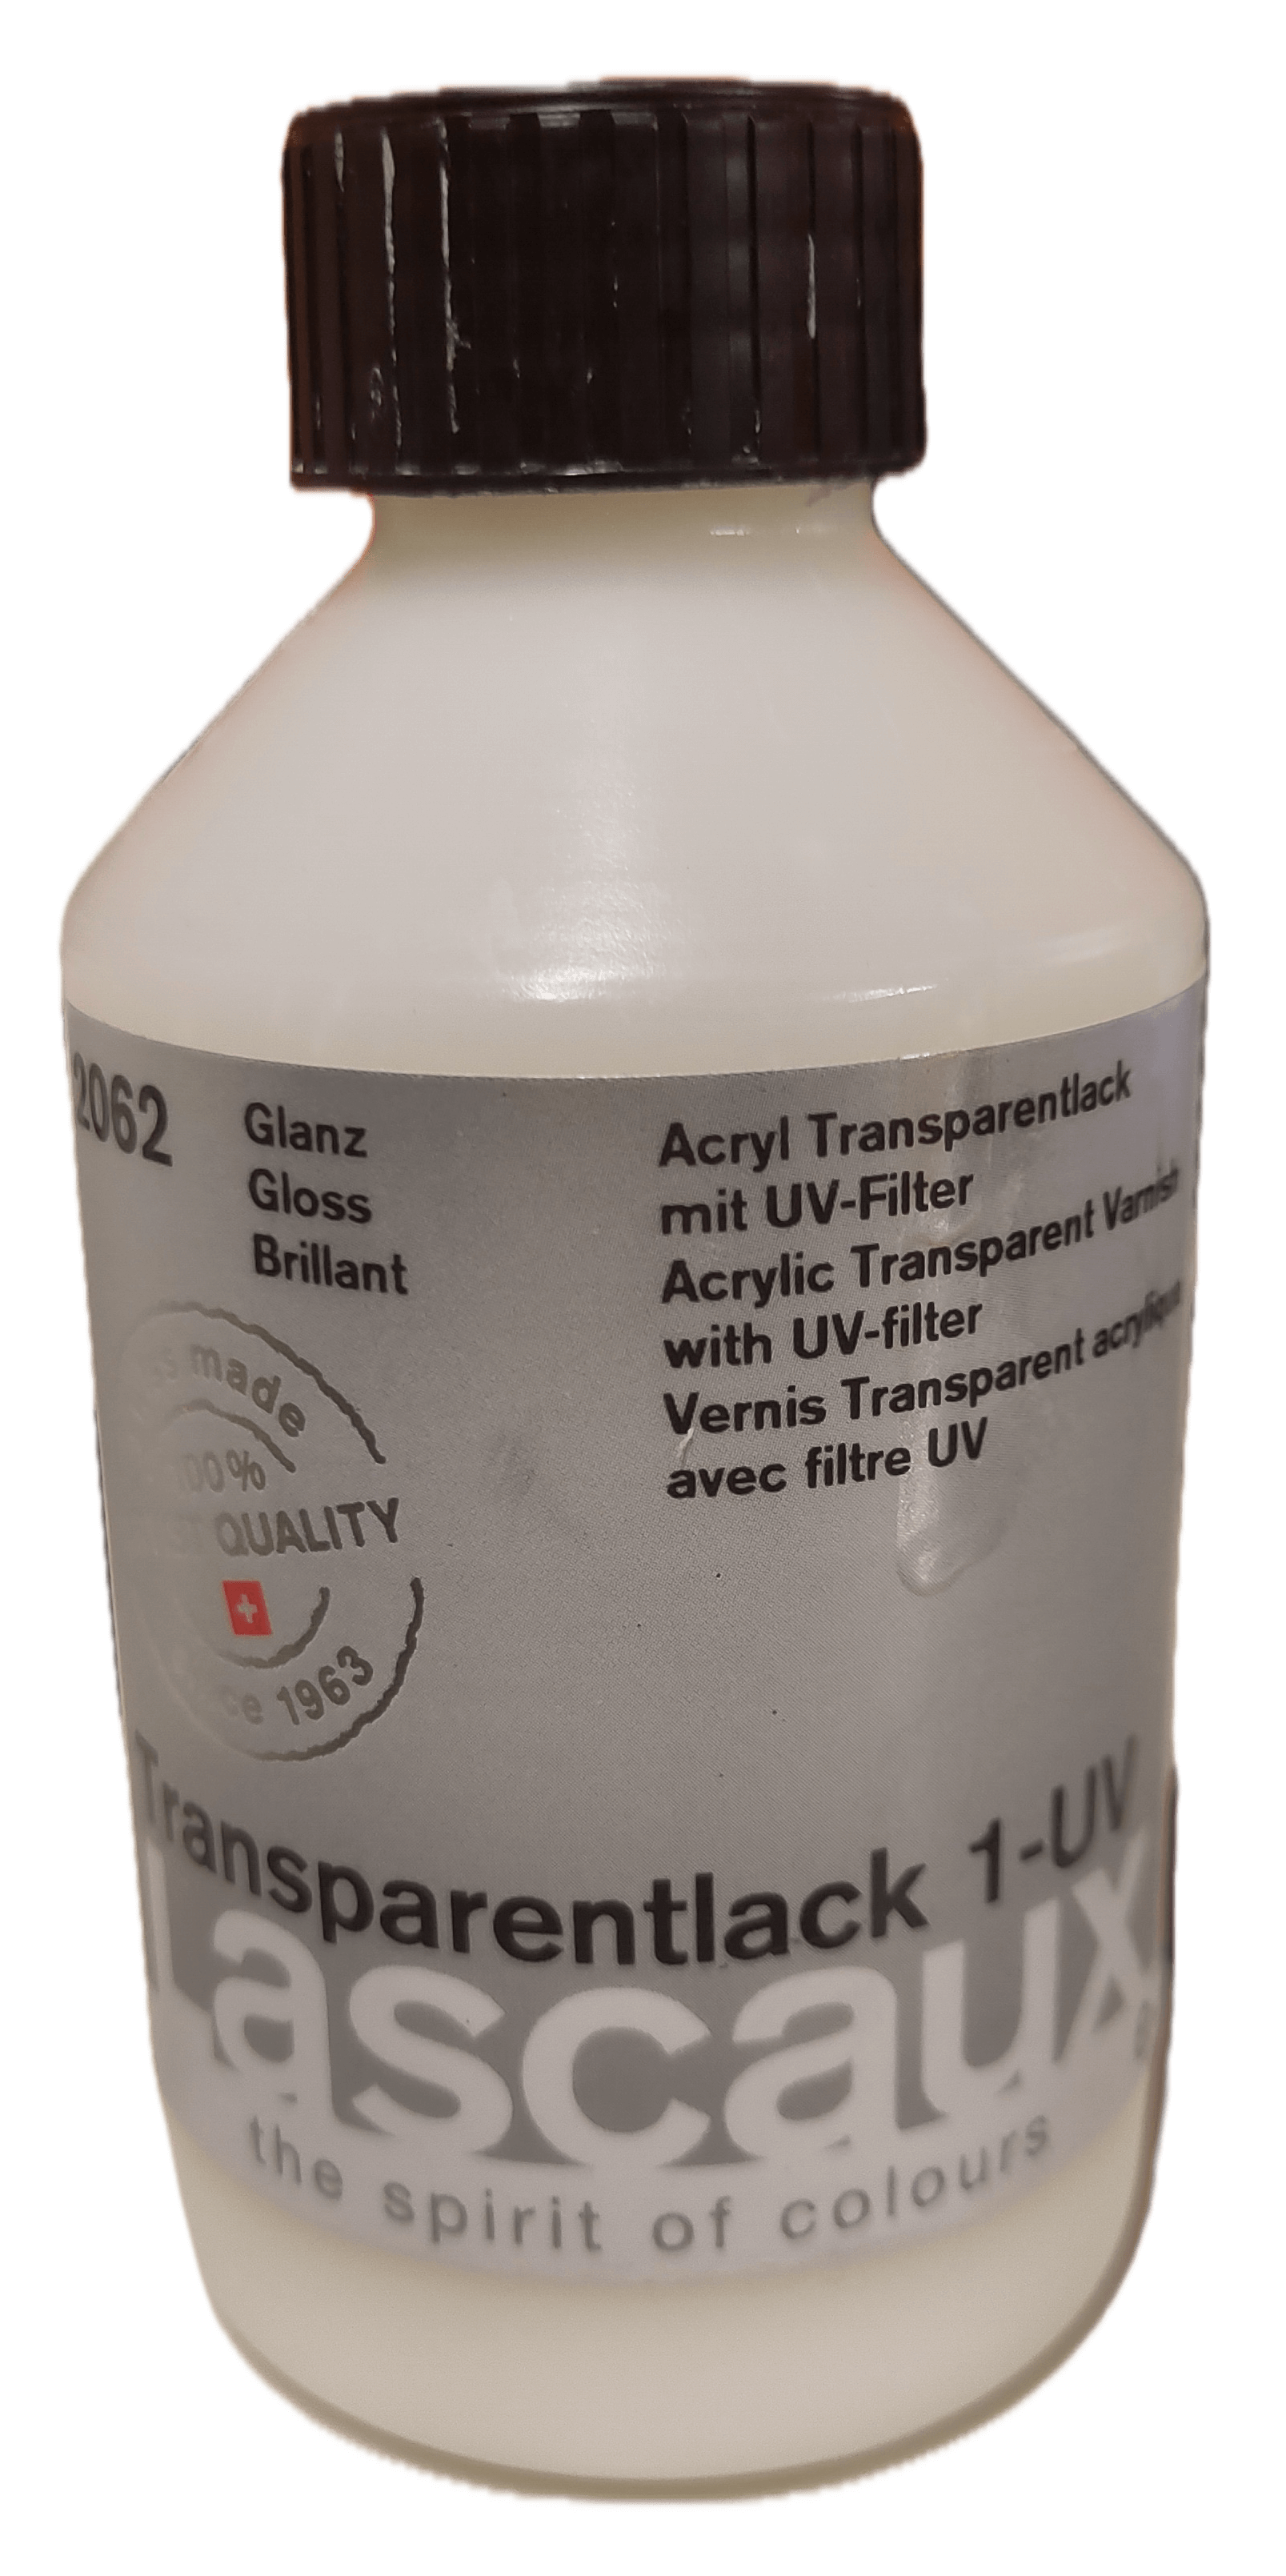
\includegraphics[width=0.3\textwidth]{assets/figures/etat_art/Lascaux_vernis_brillant.png}
    \caption[Vernis Lascaux transparant et brillant]{Vernis Lascaux transparent et brillant}
\end{figure}
\footnotetext{\url{https://lascaux.ch/lascaux-varnishes-and-fixative/lascaux-transparent-varnish-1-uv-gloss}}
Le vernis est diluable avec de l'eau (ratio 4:1), résiste à l'eau et aux rayures lorsqu'il est sec. Étant fabriqué à base d'eau,
l'aérosol produit par ce dernier est non inflammable et peu nocif (peut provoquer une réaction allergique sur la peau: warning H317).

Comme dit dans la fiche technique du vernis (\ref{fiche_technique_Lascaux}), ce matériau peut s'appliquer autant avec un \say{pistolet à peinture} qu'avec
un pinceau, ce qui correspond à notre champ d'application. Il faut toutefois relever que la version utilisée est la \textbf{1-UV}, cette dernière nécessite d'être
bien secouée (ou mélangé) avant d'être employée et doit être bien secouée toutes les deux minutes de spray (\ref{fiche_technique_Lascaux_UV}), le produit lorsqu'il a séché
peut être nettoyé à l'aide d'alcool isopropylique et si la buse de spray se bouche, il est recommandé d'utiliser de l'acétone.

% Please add the following required packages to your document preamble:
% \usepackage{graphicx}
% \usepackage[table,xcdraw]{xcolor}
% Beamer presentation requires \usepackage{colortbl} instead of \usepackage[table,xcdraw]{xcolor}
\begin{table}[H]
    \centering
    \resizebox{\textwidth}{!}{%
        \begin{tabular}{|c|c|}
            \hline
            Avantages                                       & Inconvénients                                                      \\ \hline
            \rowcolor[HTML]{92FAA4}
            Fiche technique bien fournie                    & \cellcolor[HTML]{EB726A}Besoin d'être secouée toutes les 2 minutes \\ \hline
            \cellcolor[HTML]{92FAA4}Diluable à l'eau        &                                                                    \\ \hline
            \cellcolor[HTML]{92FAA4}Non-toxique             &                                                                    \\ \hline
            \cellcolor[HTML]{92FAA4}Non inflammable         &                                                                    \\ \hline
            \cellcolor[HTML]{92FAA4}Projetable au spray gun &                                                                    \\ \hline
        \end{tabular}%
    }
    \caption{Table des avantages et inconvénients du vernis Lascaux}
    \label{tab:lascaux_UV}
\end{table}

\newpage
\subsection{Vernis acrylique transparent d'Amsterdam}
Là encore, c'est un des liquides hérités de la boîte de matériel. C'est un vernis acrylique transparent et brillant de la marque \href{https://www.amsterdam-acrylics.com/fr/}{Amsterdam} dont la composition
n'est pas à base d'eau.
\begin{figure}[H]
    \centering
    \begin{subfigure}{.5\textwidth}
        \centering
        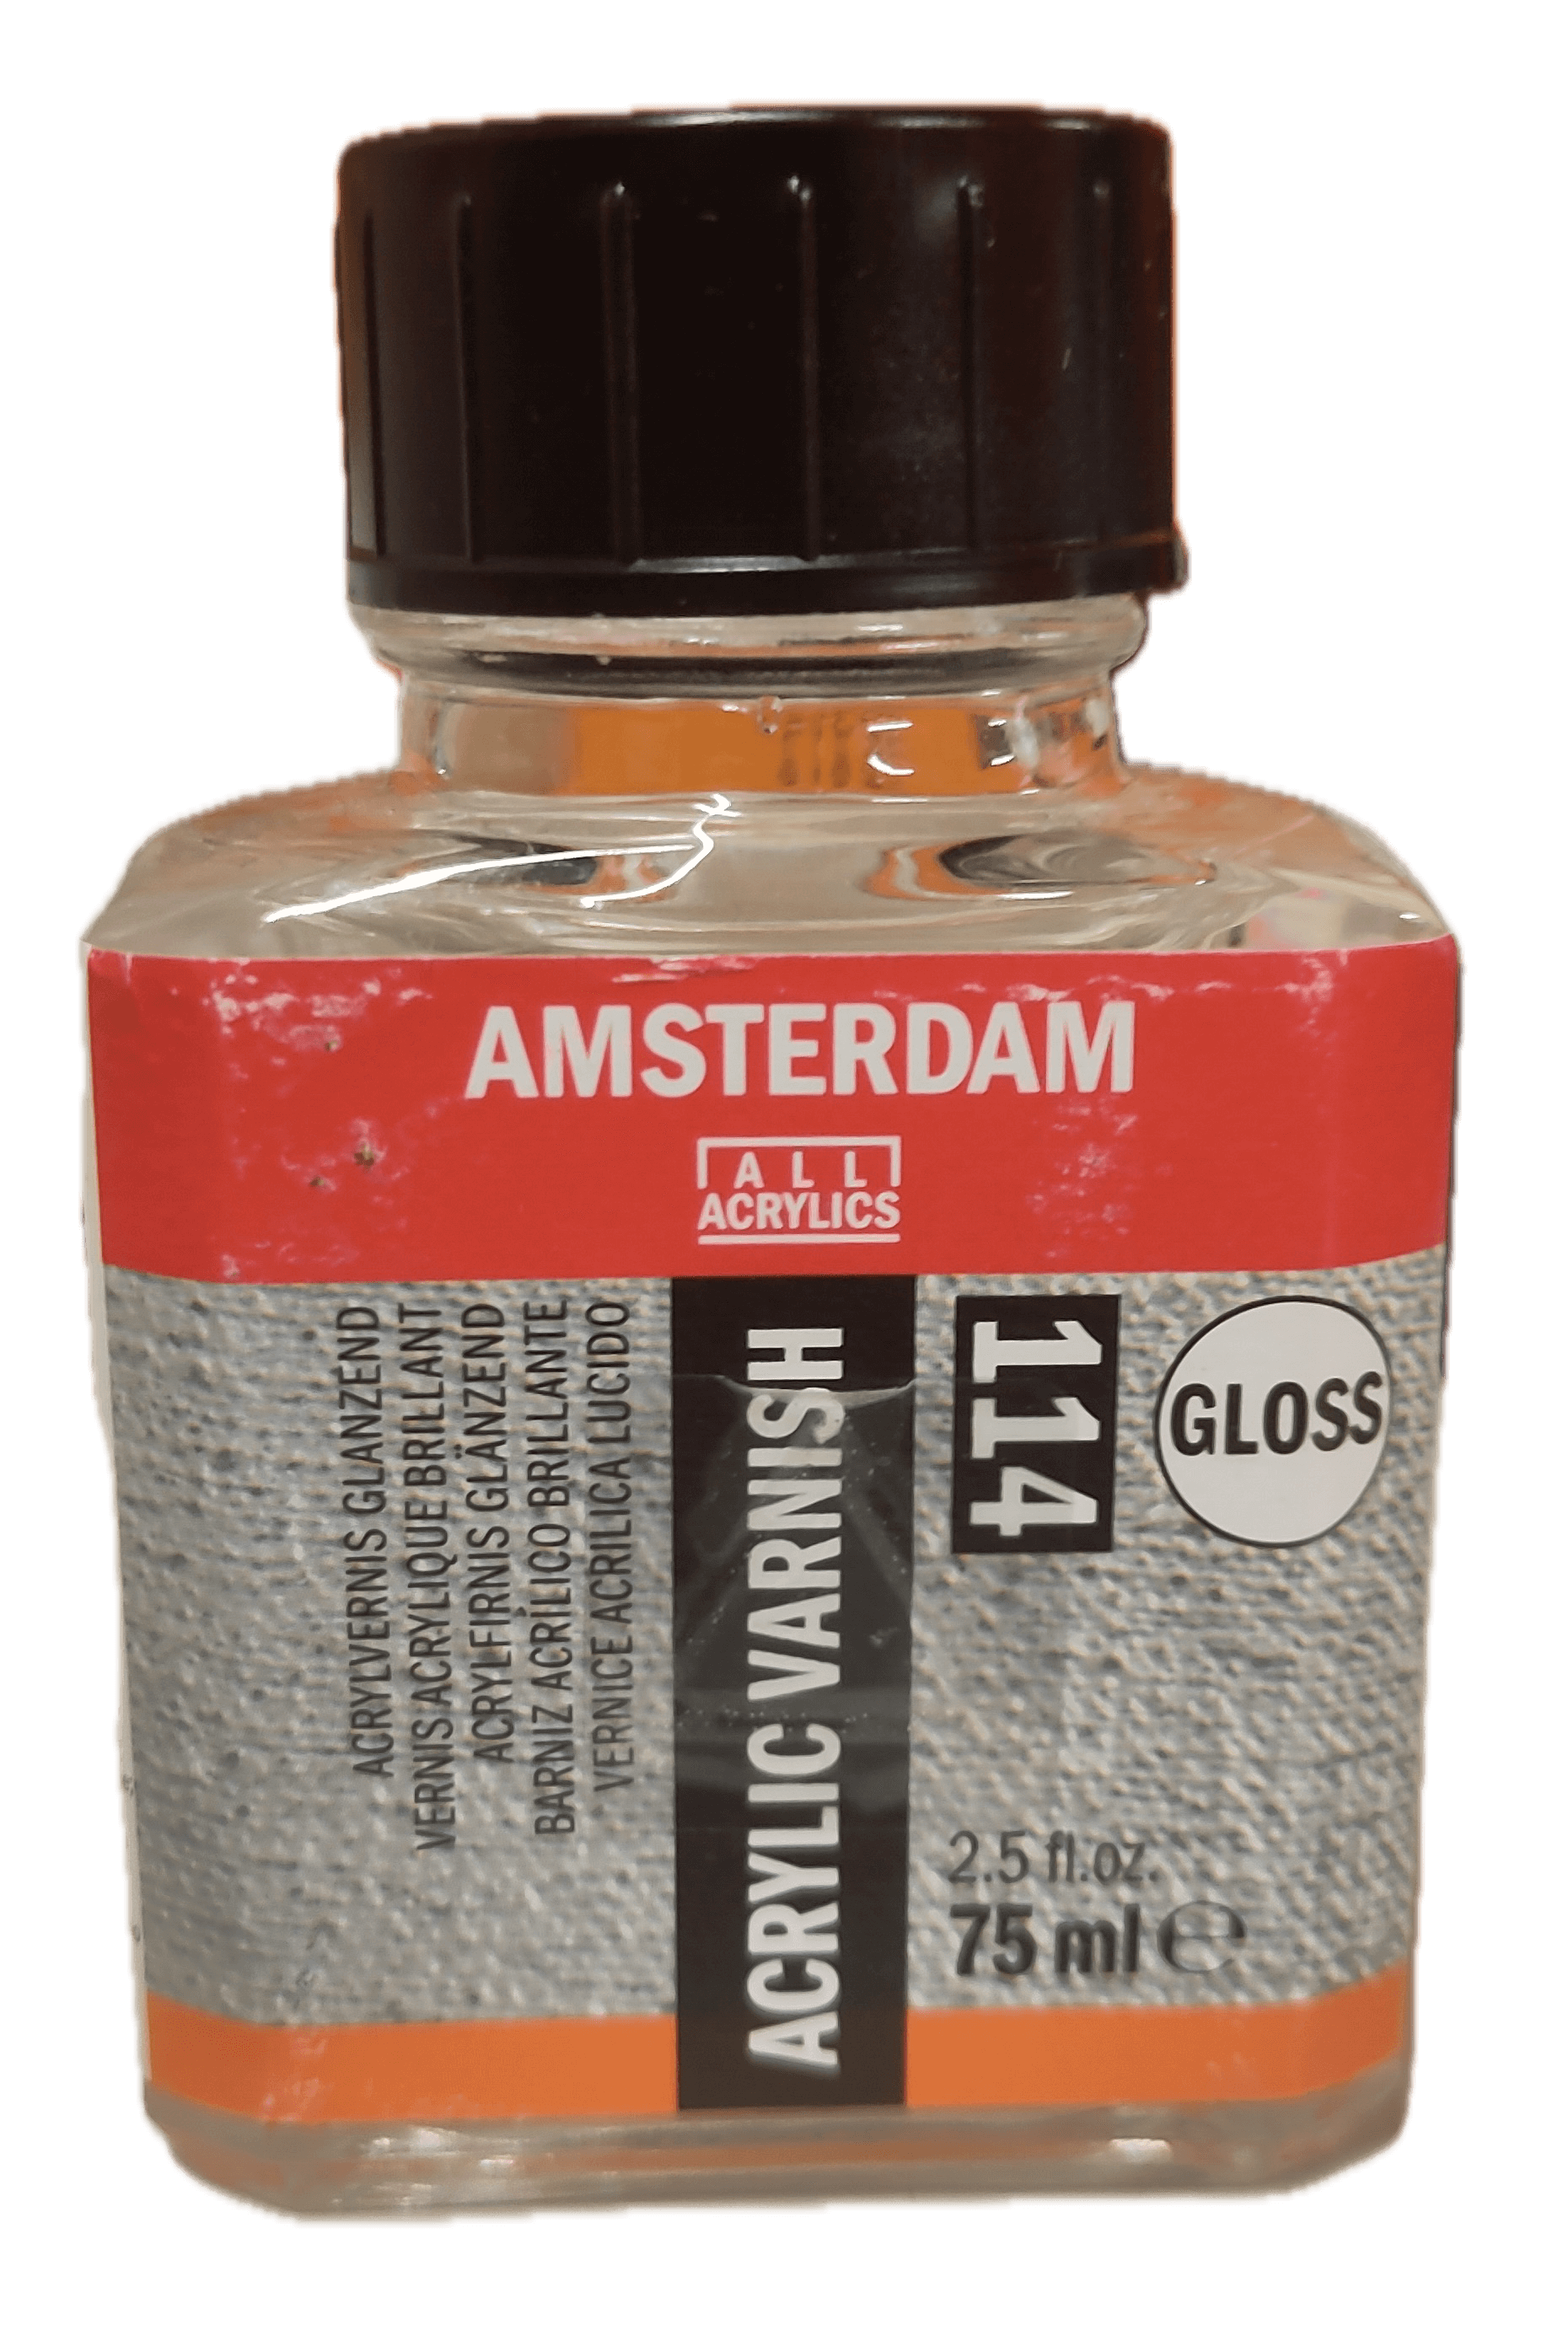
\includegraphics[width=0.6\linewidth]{assets/figures/etat_art/Amsterdam_vernis_acrylique.png}
        \caption{Robotisation de la position de l'aiguille}
        \label{fig:vernis_amsterdam_front}
    \end{subfigure}%
    \begin{subfigure}{.5\textwidth}
        \centering
        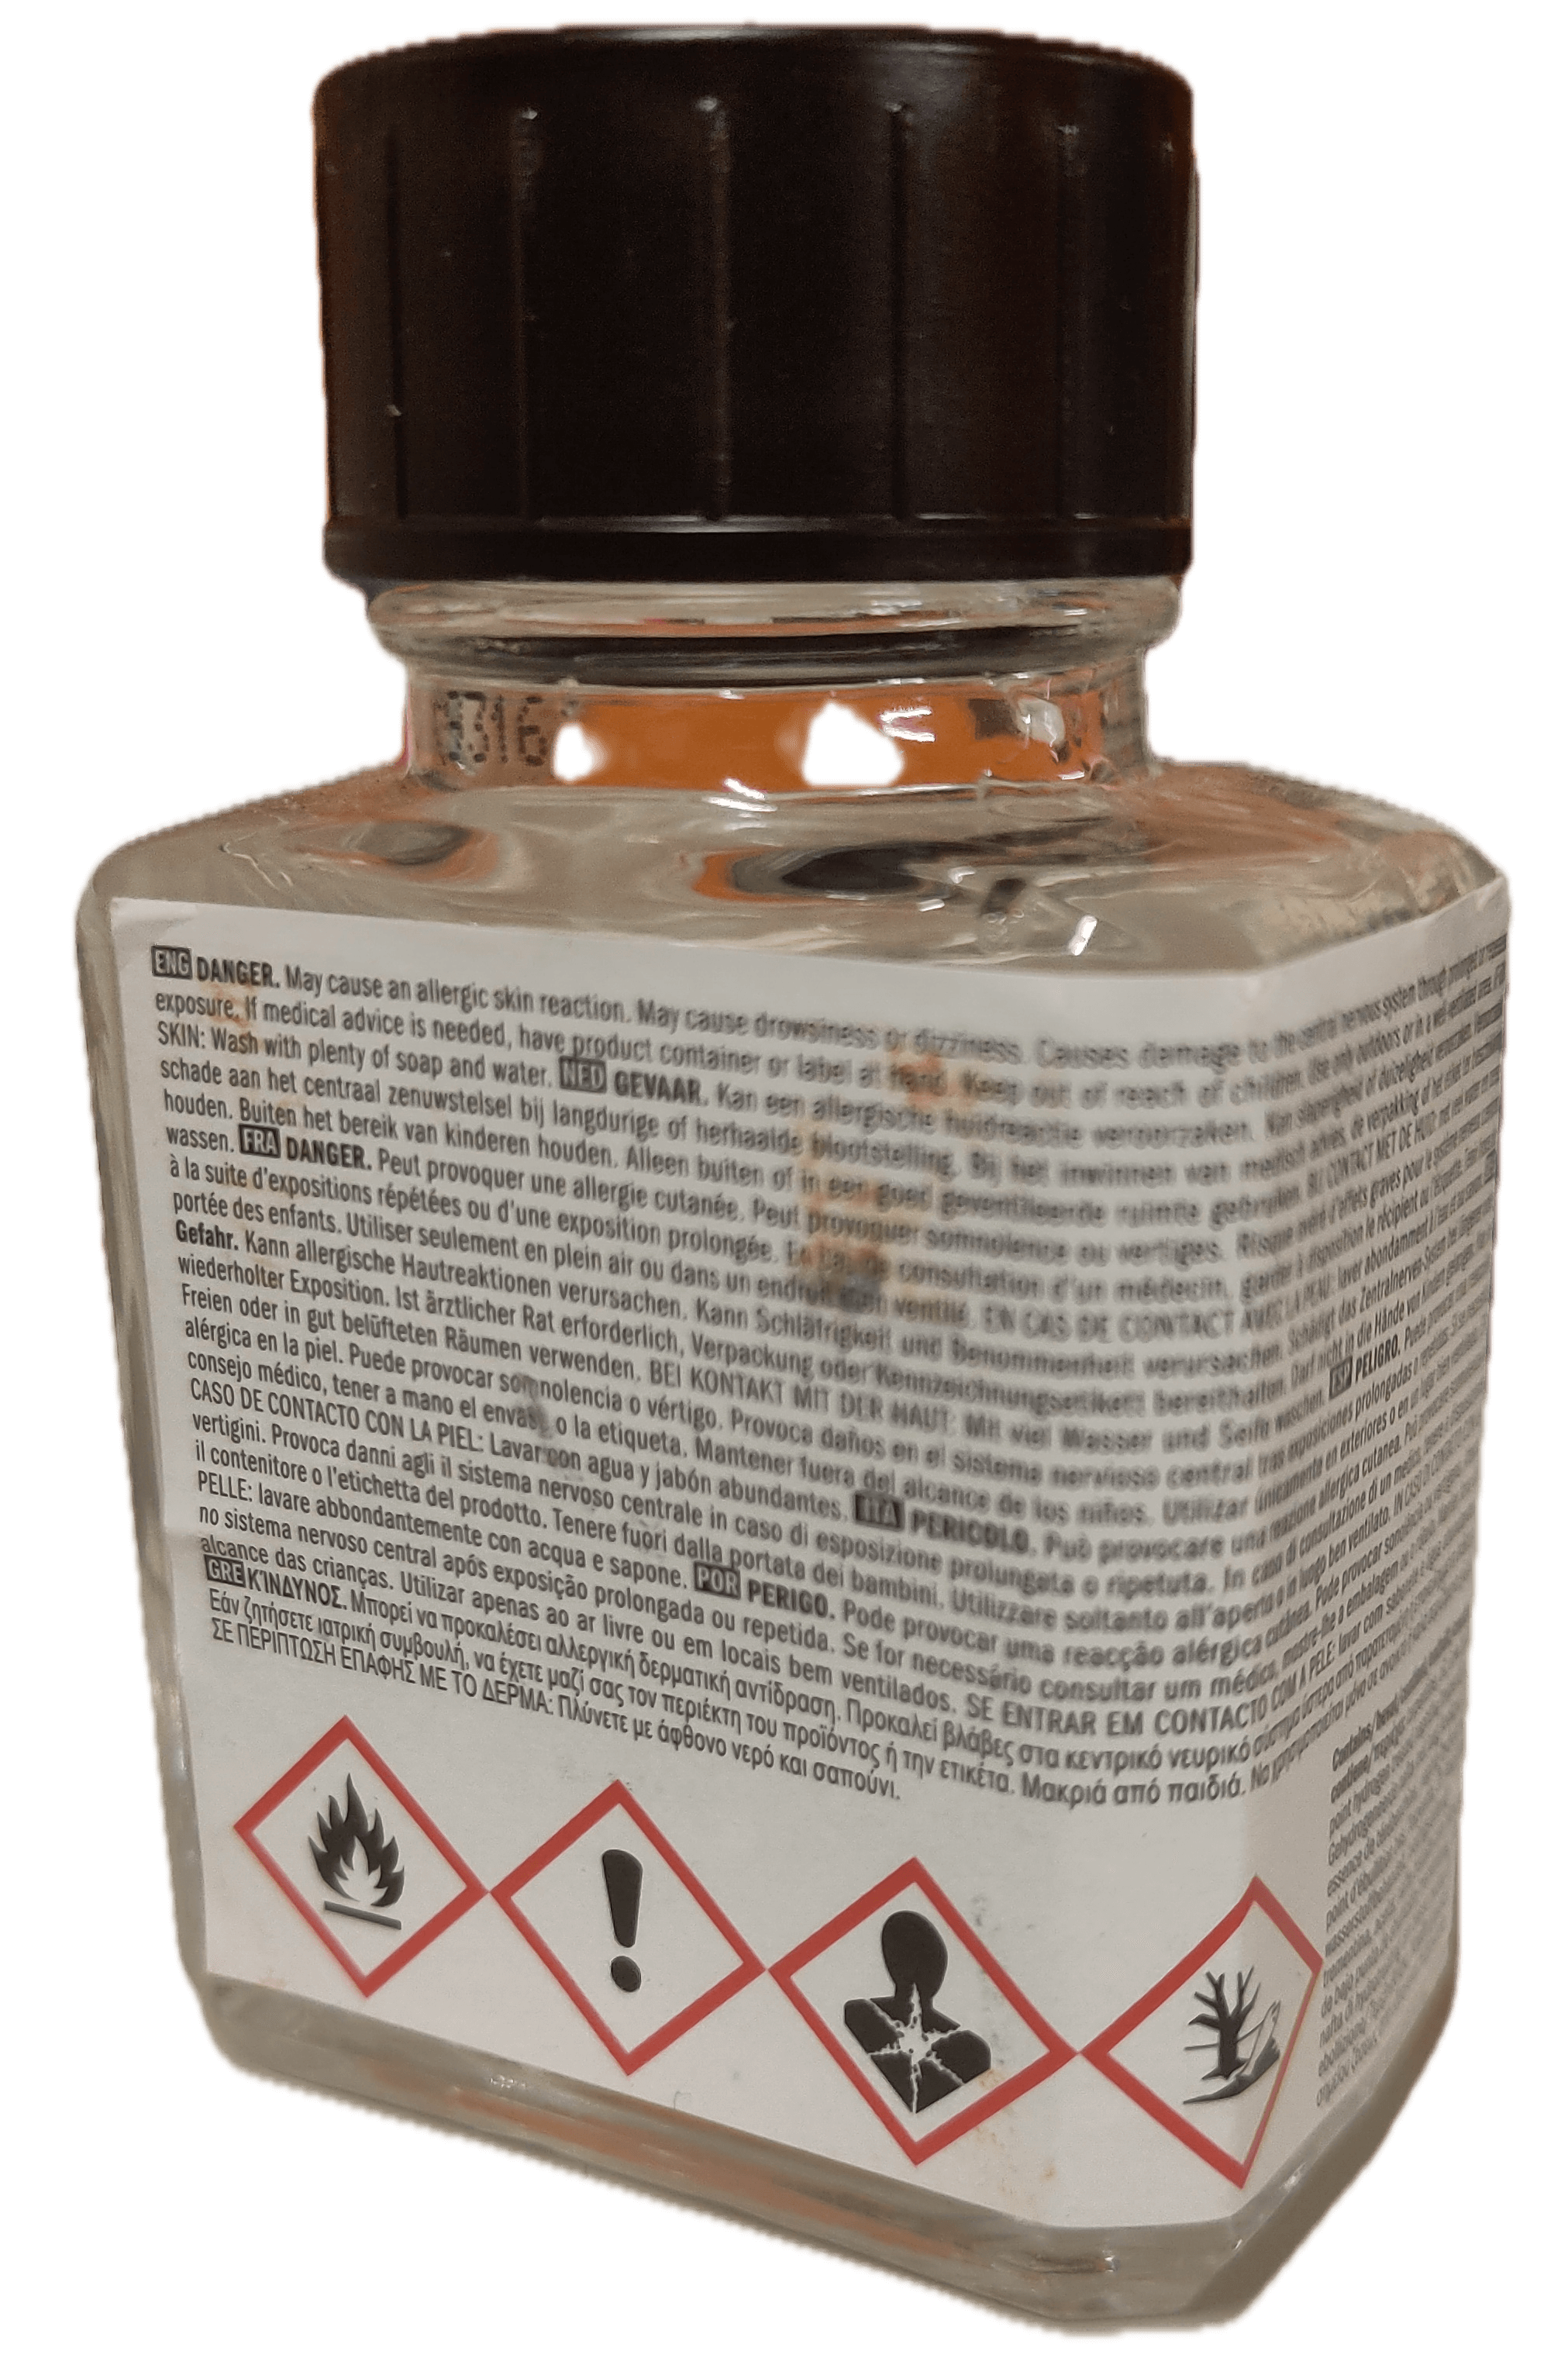
\includegraphics[width=0.6\linewidth]{assets/figures/etat_art/Amsterdam_vernis_acrylique_dos.png}
        \caption{Robotisation du bouton d'activation du spray}
        \label{fig:vernis_amsterdam_dos}
    \end{subfigure}
    \caption{Différentes robotisations de la machine originale}
    \label{fig:Vernis_amsterdam_photos}
\end{figure}
La \href{https://www.amsterdam-acrylics.com/fr/catalogue/amsterdam-protection/vernis-acrylique-brillant-flacon-250ml/}{page produit}\footnotemark est beaucoup moins fournie en détails que celle du vernis Lascaux
\footnotetext{\url{https://www.amsterdam-acrylics.com/fr/catalogue/amsterdam-protection/vernis-acrylique-brillant-flacon-250ml/}}, il est possible d'apprendre que le vernis est diluable dans de l'essence de pétrole, que le produit
sec est nettoyable aussi à l'essence de pétrole, qu'il s'applique de préférence avec un pinceau, que comme vu sur la \autoref{fig:vernis_amsterdam_dos} il est: irritant, allergène, toxique pour les organismes aquatiques, peut déclencher
des vertiges, il est cancérigène, mais surtout il est extrêmement inflammable surtout en aérosol.

Pour résumer, ce produit est déjà nocif dans sa forme liquide à appliquer au pinceau, il semble alors que le transformer en milliers de petites gouttelettes microscopiques très facilement respirables et se déposant partout
n'est pas la meilleure des idées.

Pour résumer les avantages et inconvénients :

% Please add the following required packages to your document preamble:
% \usepackage{graphicx}
% \usepackage[table,xcdraw]{xcolor}
% Beamer presentation requires \usepackage{colortbl} instead of \usepackage[table,xcdraw]{xcolor}
\begin{table}[H]
    \centering
    \resizebox{\textwidth}{!}{%
        \begin{tabular}{|c|c|}
            \hline
            Avantages                        & Inconvénients                                                                 \\ \hline
            \rowcolor[HTML]{92FAA4}
            Transparent sous forme liquide   & \cellcolor[HTML]{EB726A}Pas de fiche technique bien documentée                \\ \hline
            \rowcolor[HTML]{92FAA4}
            Pas besoin de secouer le liquide & \cellcolor[HTML]{EB726A}Pas de précision quant à l'utilisation d'un spray gun \\ \hline
            \rowcolor[HTML]{FFFFFF}
                                             & \cellcolor[HTML]{EB726A}Toxique                                               \\ \hline
            \rowcolor[HTML]{FFFFFF}
                                             & \cellcolor[HTML]{EB726A}Extrêmement inflammable                               \\ \hline
        \end{tabular}%
    }
    \caption{Résumé des avantages et inconvénients du vernis Amsterdam}
    \label{tab:Amsterdam_vernis}
\end{table}

\newpage
\subsection{Vernis acrylique transparent pour aérographe de chez StardustColors}

À partir de maintenant, tous les matériaux de projection présentés ne viennent pas de la boîte d'équipement de la machine.
Le vernis transparent acrylique "top coat" de chez \href{https://www.stardustcolors.co.uk/}{Stardust Colors} est un produit spécialisé
pour la projection à l'aide d'un aérographe (et méthodes analogues) et selon la \href{https://www.stardustcolors.co.uk/stardust-acrylic-pro-series/1270-airbrush-acrylic-polyurethane-topcoats-matt-satin-or-gloss-3700730801942.html}{page produit}\footnotemark
\footnotetext{\url{https://www.stardustcolors.co.uk/stardust-acrylic-pro-series/1270-airbrush-acrylic-polyurethane-topcoats-matt-satin-or-gloss-3700730801942.html}}, le produit ne nécessite même pas de dilution pour les têtes de buses jusqu'à 0.2mm de diamètre,
pour diluer ce vernis, le fabricant propose des "thinners" propriétaires et donc à la composition inconnue, il est tout de même précisé dans la datasheet des produits \autoref{fiche_technique_Stardust}
que la composition des vernis est à base d'eau et qu'elle est non toxique (malgré tout ils recommandent l'utilisation d'un masque).

\begin{figure}[H]
    \centering
    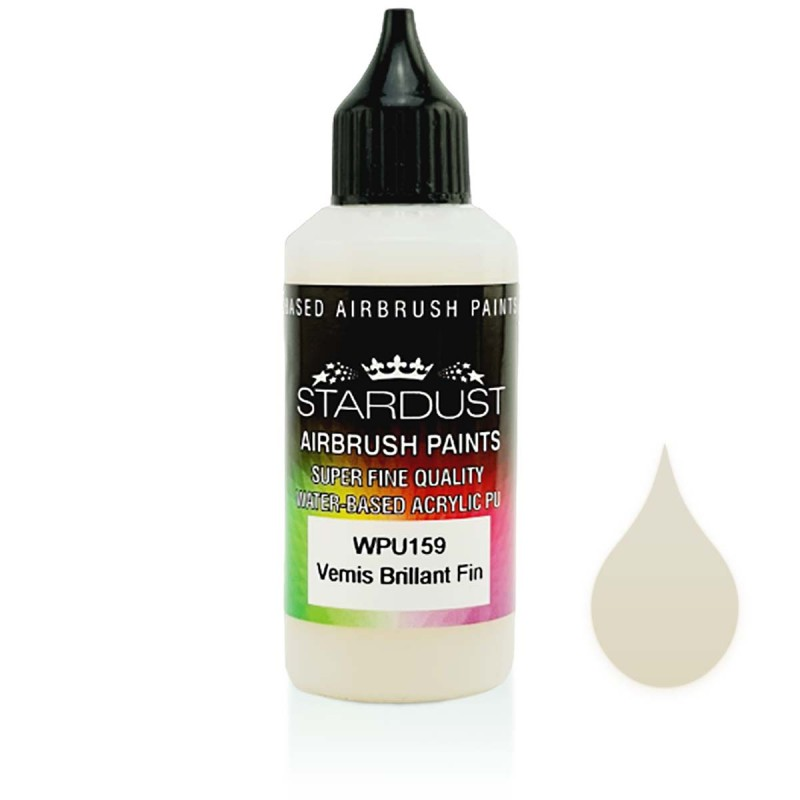
\includegraphics[width=0.5\textwidth]{assets/figures/etat_art/Stardust_vernis.jpg}
    \caption[Vernis transparent brillant Stardust Colors]{Vernis transparent brillant Stardust Colors\cite{Bouteille_vernis_stardust}}
\end{figure}
À noter que ce produit semble difficilement trouvable en suisse, il conviendrait donc de l'importer en cas de commande.
% Please add the following required packages to your document preamble:
% \usepackage{graphicx}
% \usepackage[table,xcdraw]{xcolor}
% Beamer presentation requires \usepackage{colortbl} instead of \usepackage[table,xcdraw]{xcolor}
\begin{table}[H]
    \centering
    \resizebox{\textwidth}{!}{%
        \begin{tabular}{|c|c|}
            \hline
            Avantages                                           & Inconvénients                                               \\ \hline
            \rowcolor[HTML]{92FAA4}
            Formule à base d'eau                                & \cellcolor[HTML]{EB726A}Difficilement obtenable en Suisse   \\ \hline
            \rowcolor[HTML]{92FAA4}
            Non toxique                                         & \cellcolor[HTML]{EB726A}Dilution avec produit propriétaire  \\ \hline
            \rowcolor[HTML]{92FAA4}
            Conçue pour la projection par aérographe            & \cellcolor[HTML]{EB726A}Nettoyage avec produit propriétaire \\ \hline
            \rowcolor[HTML]{92FAA4}
            Une fiche technique adéquatement fournie disponible & \cellcolor[HTML]{FFFFFF}                                    \\ \hline
        \end{tabular}%
    }
    \caption{Résumé des avantages et inconvénients du vernis Stardust}
    \label{tab:Stardust_vernis}
\end{table}
\newpage
\subsection{Vernis acrylique transparent pour aérographe de Createx}
C'est un produit aux propriétés similaires à celle du produit de Stardust Colors, il a par contre une fiche technique très fournie \autoref{fiche_technique_Createx} et est \href{https://www.airbrush-shop.ch/contents/de-ch/p6000.html}{obtenable} en Suisse.
\begin{figure}[H]
    \centering
    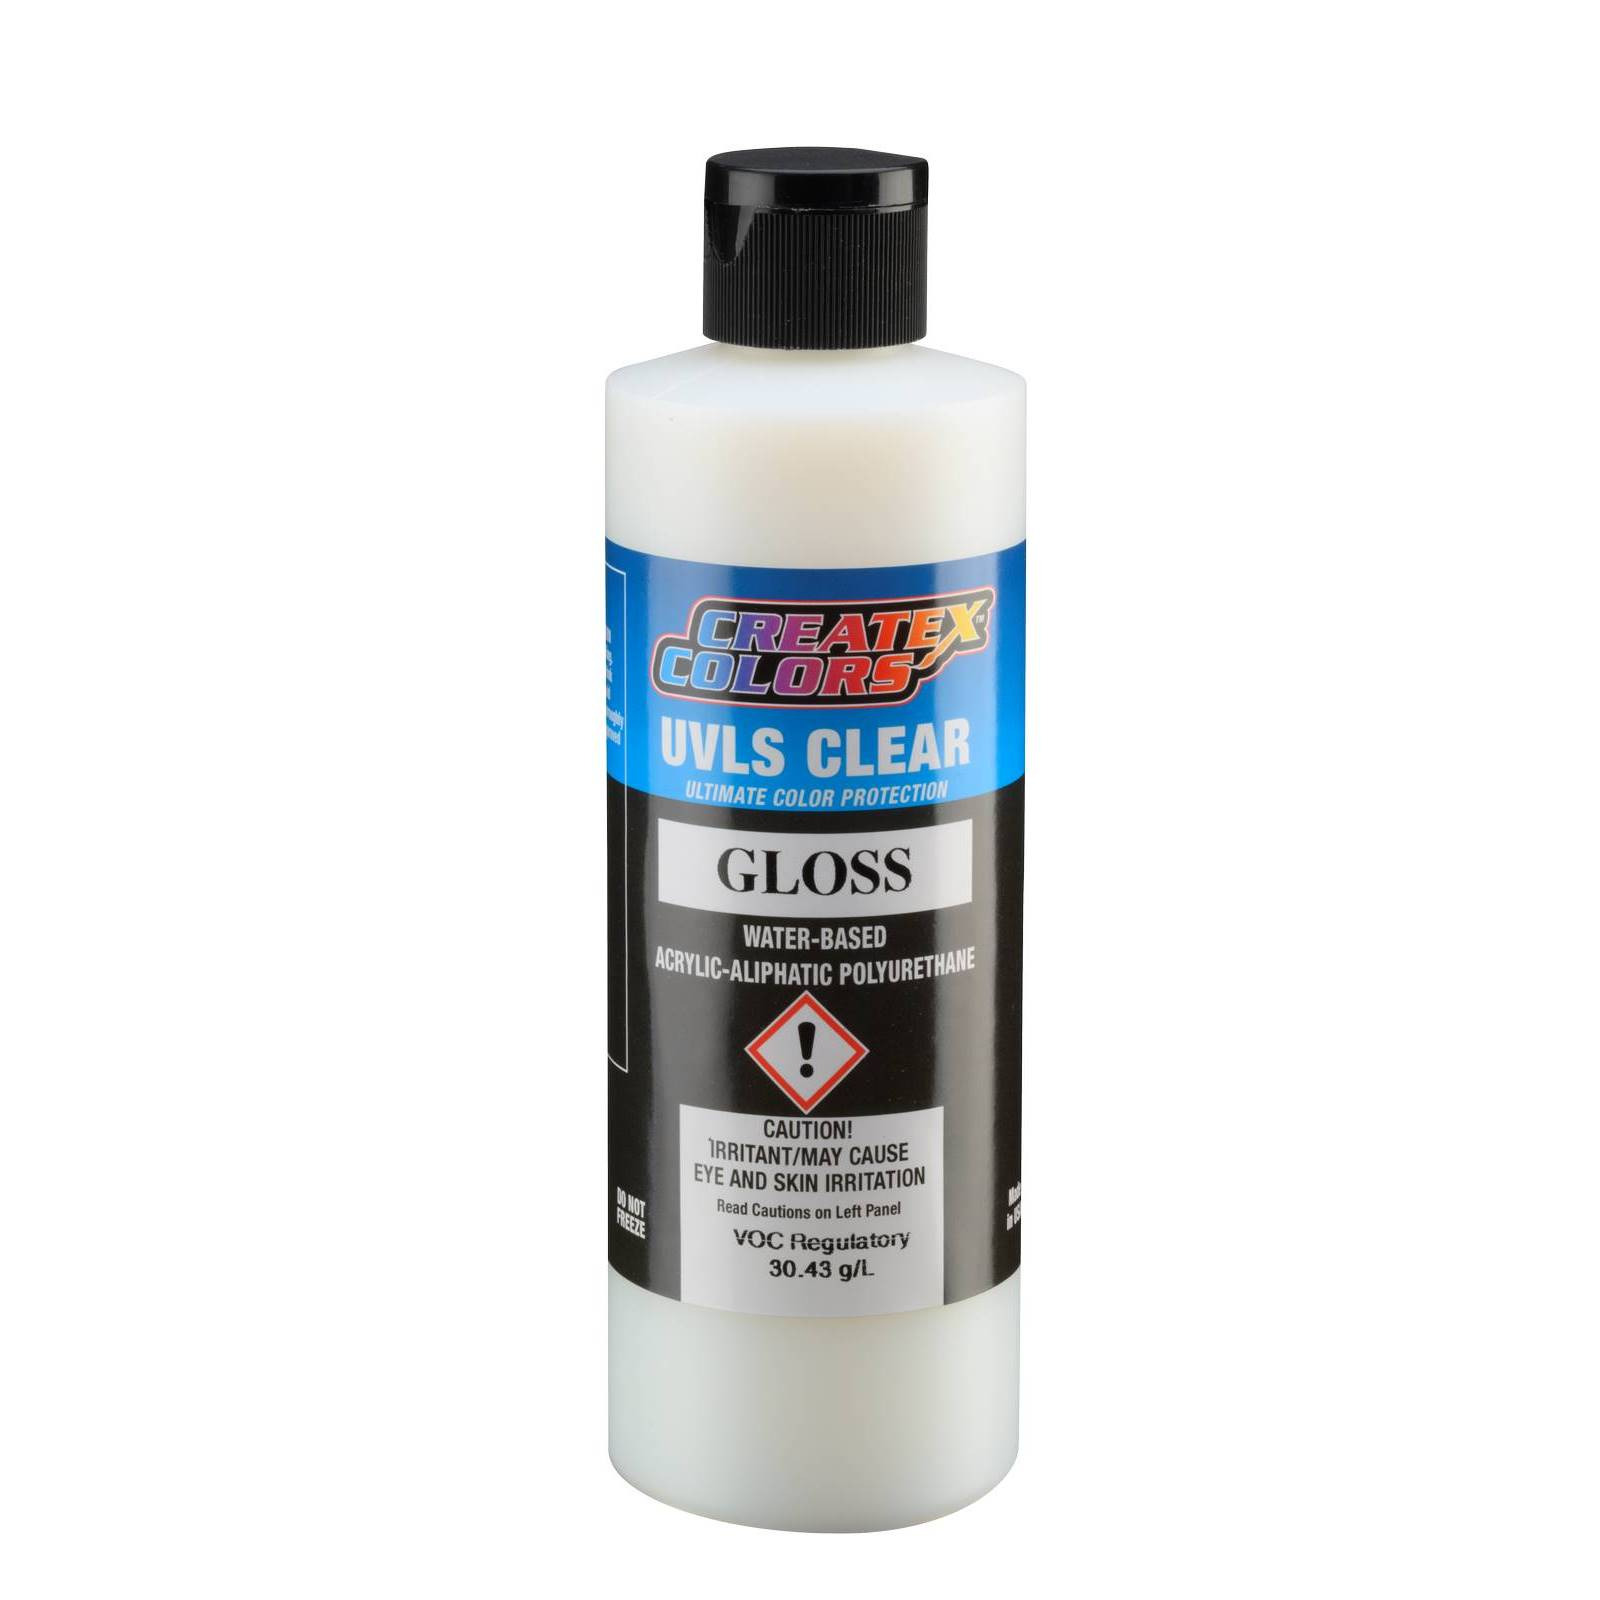
\includegraphics[width=0.45\textwidth]{assets/figures/etat_art/Createx_bouteille.jpg}
    \caption[Vernis transparent brillant Createx]{Vernis transparent brillant Createx\cite{Bouteille_Createx}}
\end{figure}
% Please add the following required packages to your document preamble:
% \usepackage{graphicx}
% \usepackage[table,xcdraw]{xcolor}
% Beamer presentation requires \usepackage{colortbl} instead of \usepackage[table,xcdraw]{xcolor}
\begin{table}[H]
    \centering
    \resizebox{\textwidth}{!}{%
        \begin{tabular}{|c|c|}
            \hline
            Avantages                                    & Inconvénients                                               \\ \hline
            \rowcolor[HTML]{92FAA4}
            Formule à base d'eau                         & \cellcolor[HTML]{EB726A}Dilution avec produit propriétaire  \\ \hline
            \rowcolor[HTML]{92FAA4}
            Non toxique                                  & \cellcolor[HTML]{EB726A}Nettoyage avec produit propriétaire \\ \hline
            \rowcolor[HTML]{92FAA4}
            Conçue pour la projection par aérographe     & \cellcolor[HTML]{FFFFFF}                                    \\ \hline
            \rowcolor[HTML]{92FAA4}
            Une fiche technique bien fournie disponible  & \cellcolor[HTML]{FFFFFF}                                    \\ \hline
            \cellcolor[HTML]{92FAA4}Disponible en Suisse & \multicolumn{1}{l|}{}                                       \\ \hline
        \end{tabular}%
    }
    \caption{Résumé des avantages et inconvénients du vernis Createx}
    \label{tab:Createx_vernis}
\end{table}
\section{Conclusion}\label{sec:conclusion_etat_art}
\subsection{Système de projection}
Au final, la solution de projection choisie est celle de la \textbf{buse d'atomisation pneumatique}, en effet, ces dernières sont
munies de connecteurs standardisés et sont grandement employées dans l'industrie, le prix peut être un frein au début, mais il faut
garder en tête que ce sont des pièces destinées aux professionnels.

\subsection{Liquide à projeter}
Le liquide à projeter sélectionné est le \textbf{vernis de chez Lascaux}, comme vu dans la \autoref{tab:lascaux_UV} il présente de nombreux avantages, dont
un avantage clef, il est disponible directement sans délais, ce sera donc le liquide utilisé dans la future machine, mais aussi celui qui a été utilisé lors de
l'étape de familiarisation avec la machine.